% DO NOT COMPILE THIS FILE DIRECTLY!
% This is included by the other .tex files.

\begin{frame}[t,plain]
\titlepage
\end{frame}

\begin{frame}{Agenda}
    \begin{itemize}
        \item Introduction to Information Sharing with MISP
        \item General MISP usage - diving into MISP functionalities and integration
        \item GSMA instance usage by Alexandre De Oliveira
        \item Q \& A
    \end{itemize}
\end{frame}

\begin{frame}
 \frametitle{MISP: Started from a practical use-case}
 \begin{itemize}
         \item During a malware analysis workgroup in 2012, we discovered that we worked on the analysis of the same malware.
         \item We wanted to share information in an easy and automated way {\bf to avoid duplication of work}.
         \item Christophe Vandeplas (then working at the CERT for the Belgian MoD) showed us his work on a platform that later became MISP.
         \item A first version of the MISP Platform was used by the MALWG and {\bf the increasing feedback of users} helped us to build an improved platform.
         \item MISP is now {\bf a community-driven development}.
 \end{itemize}
\end{frame}

\begin{frame}
\frametitle{about CIRCL}
The Computer Incident Response Center Luxembourg (CIRCL) is a government-driven initiative designed to provide a systematic response facility to computer security threats and incidents. CIRCL is the CERT for the private sector, communes and non-governmental entities in Luxembourg and is operated by securitymadein.lu g.i.e.
\end{frame}

\begin{frame}
\frametitle{MISP and CIRCL}
\begin{itemize}
\item CIRCL is mandated by the Ministry of Economy and acting as the Luxembourg National CERT for private sector.
\item CIRCL leads the development of the Open Source MISP threat intelligence platform which is used by many military or intelligence communities, private companies, financial sector, National CERTs and LEAs globally.
\item {\bf CIRCL runs multiple large MISP communities performing active daily threat-intelligence sharing}.
\end{itemize}
\begin{center}
    
\includegraphics{en_cef.png}
\end{center}
\end{frame}

\begin{frame}
\frametitle{Many objectives from different user-groups}
    \begin{itemize}
        \item Sharing indicators for a {\bf detection} matter.
            \begin{itemize}
                \item \textit{Do I have infected systems in my infrastructure or the ones I operate?}
            \end{itemize}
    \item Sharing indicators to {\bf block}.
            \begin{itemize}
                \item \textit{I use these attributes to block, sinkhole or divert traffic}
            \end{itemize}
    \item Sharing indicators to {\bf perform intelligence}.
            \begin{itemize}
                \item Gathering information about campaigns and attacks. \textit{Are they related? Who is targeting me? Who are the adversaries?}
            \end{itemize}
        \end{itemize}
        
        \vspace{1em}
        \begin{center}
        $\rightarrow$ These objectives can be {\bf conflicting}

        (e.g. False-positives have different impacts)
        \end{center}
    \end{frame}

\begin{frame}
\frametitle{Sharing Difficulties}
        \begin{itemize}
                \item Sharing difficulties are not really technical issues but often it's a matter of {\bf social interactions} (e.g. {\bf trust}).
                \item Legal restriction\footnote{\url{https://www.misp-project.org/compliance/}}
                        \begin{itemize}
                                \item \textit{Our legal framework doesn't allow us to share information}
                                \item \textit{Risk of information-leak is too high and it's too risky for our organization or partners.}
                        \end{itemize}
                \item Practical restriction
                        \begin{itemize}
                                \item \textit{We don't have information to share.}
                                \item \textit{We don't have time to process or contribute indicators.}
                                \item \textit{Our model of classification doesn't fit your model.}
                                \item \textit{Tools for sharing information are tied to a specific format, we use a different one.}
                        \end{itemize}
        \end{itemize}
\end{frame}


\begin{frame}
    \frametitle{MISP Project Overview}
    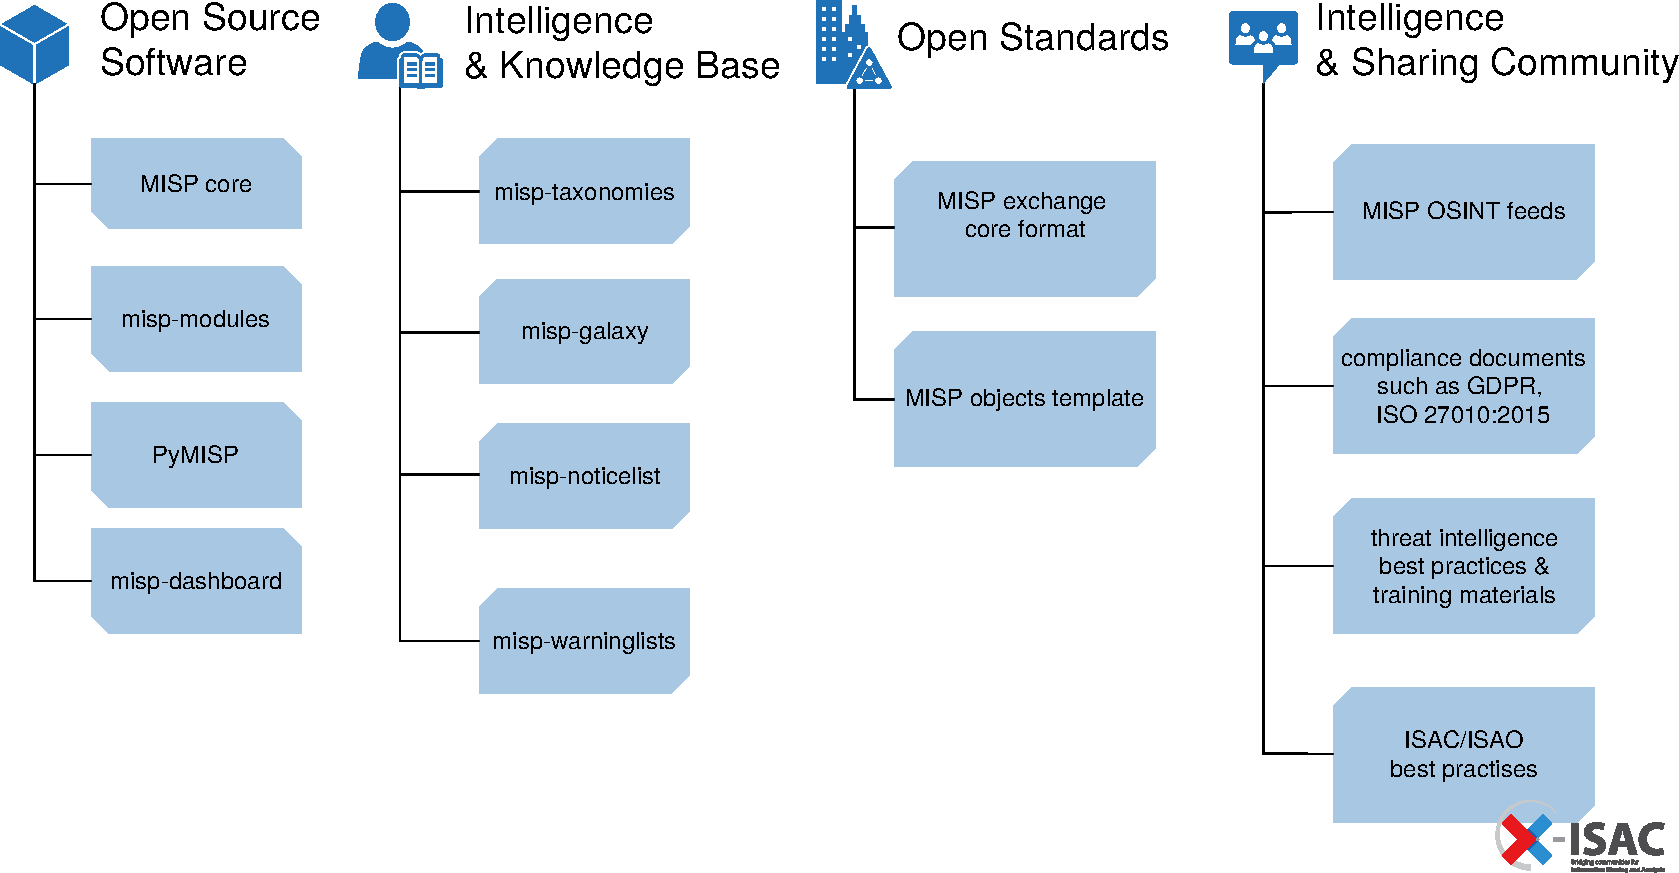
\includegraphics[scale=0.35]{misp-overview-simplified.pdf}
\end{frame}

\begin{frame}
    \frametitle{MISP model of governance}
    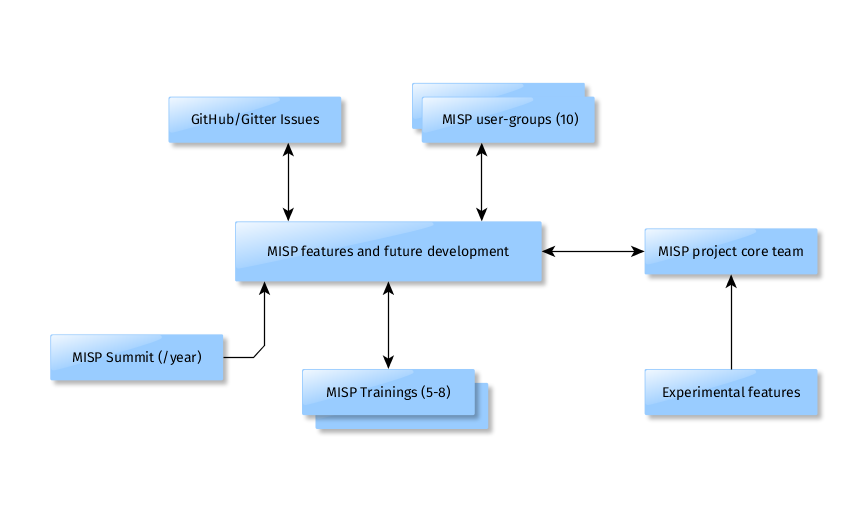
\includegraphics[scale=0.4]{governance.png}
\end{frame}

\begin{frame}
    \frametitle{Getting some naming conventions out of the way...}
     \begin{itemize}
            \item Data layer
            \begin{itemize}
                \item {\bf Events} are encapsulations for contextually linked information
                \item {\bf Attributes} are individual data points, which can be indicators or supporting data.
                \item {\bf Objects} are custom templated Attribute compositions
                \item {\bf Object references} are the relationships between other building blocks
            \end{itemize}
    \end{itemize}
\end{frame}

\begin{frame}
    \frametitle{Getting some naming conventions out of the way...}
     \begin{itemize}
            \item Context layer
            \begin{itemize}
                \item {\bf Tags} are labels attached to events/attributes and can come from {\bf Taxonomies}
                \begin{itemize}
                    \item \texttt{Android Malware}, \texttt{C2}, ...
                \end{itemize}

                \item {\bf Taxonomies} are a set of common classification allowing to express the same vocabulary among a distributed set of users and organisations 
                \begin{itemize}
                    \item \texttt{tlp:green}, \texttt{false-positive:risk="high"}, \texttt{gsma-fraud:technical="sim-card-cloning"}, \texttt{gsma-attack-category:spoofing}
                \end{itemize}

                \item {\bf Galaxy-clusters} are knowledge base items used to label events/attributes and come from {\bf Galaxies}. Basically a taxonomy with additional meta-information.
                \begin{itemize}
                    \item Typical {\bf Galaxy-clusters}: {\bf threat actors}, {\bf preventive measures}, ...
                    \item \texttt{misp-galaxy:bhadra-framework="Billing frauds"}, \texttt{misp-galaxy:bhadra-framework="DNS-based attacks"}, \texttt{misp-galaxy:threat-actor="APT 29"}
                \end{itemize}
            \end{itemize}
    \end{itemize}
\end{frame}

\begin{frame}
        \frametitle{A rich data-model: telling stories via relationships}
        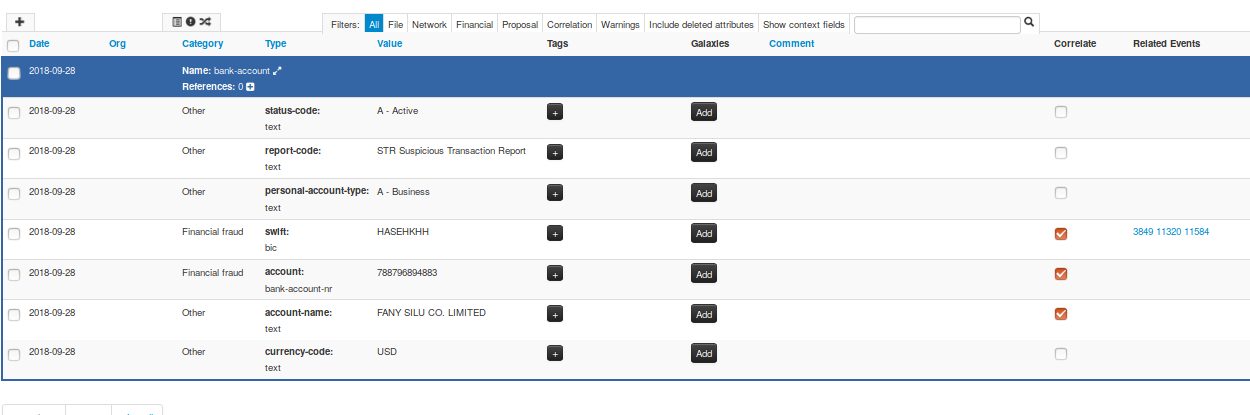
\includegraphics[scale=0.25]{screenshots/bankaccount.png}
        \begin{center}
            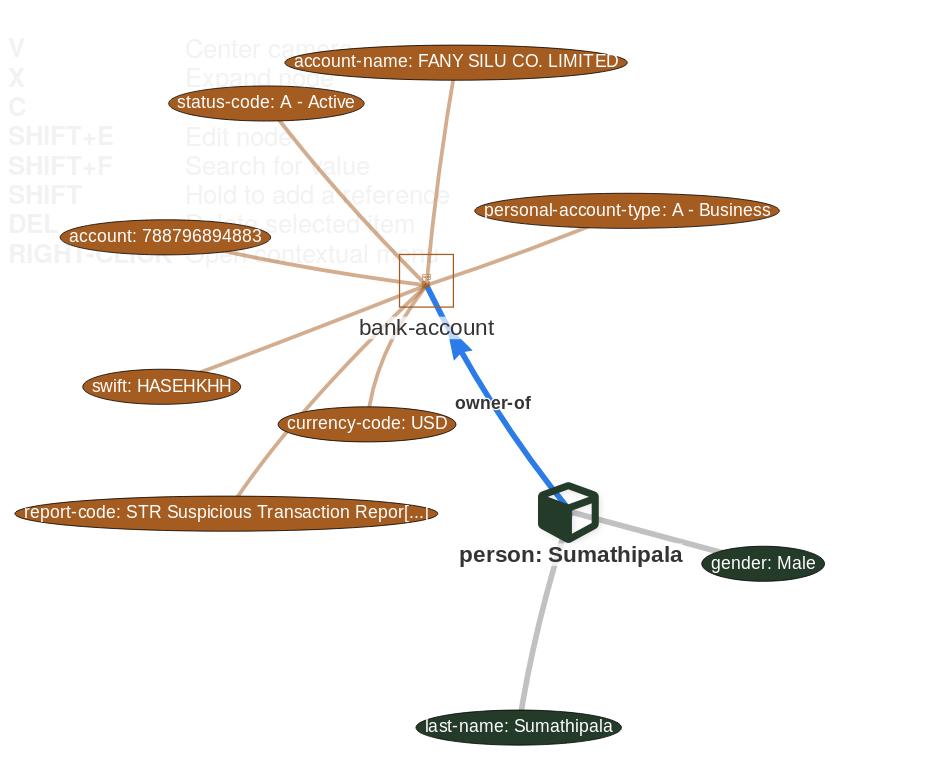
\includegraphics[scale=0.18]{screenshots/bankview.png}
        \end{center}
\end{frame}

\begin{frame}
        \frametitle{Correlation features: a tool for analysts}
        \begin{center}
            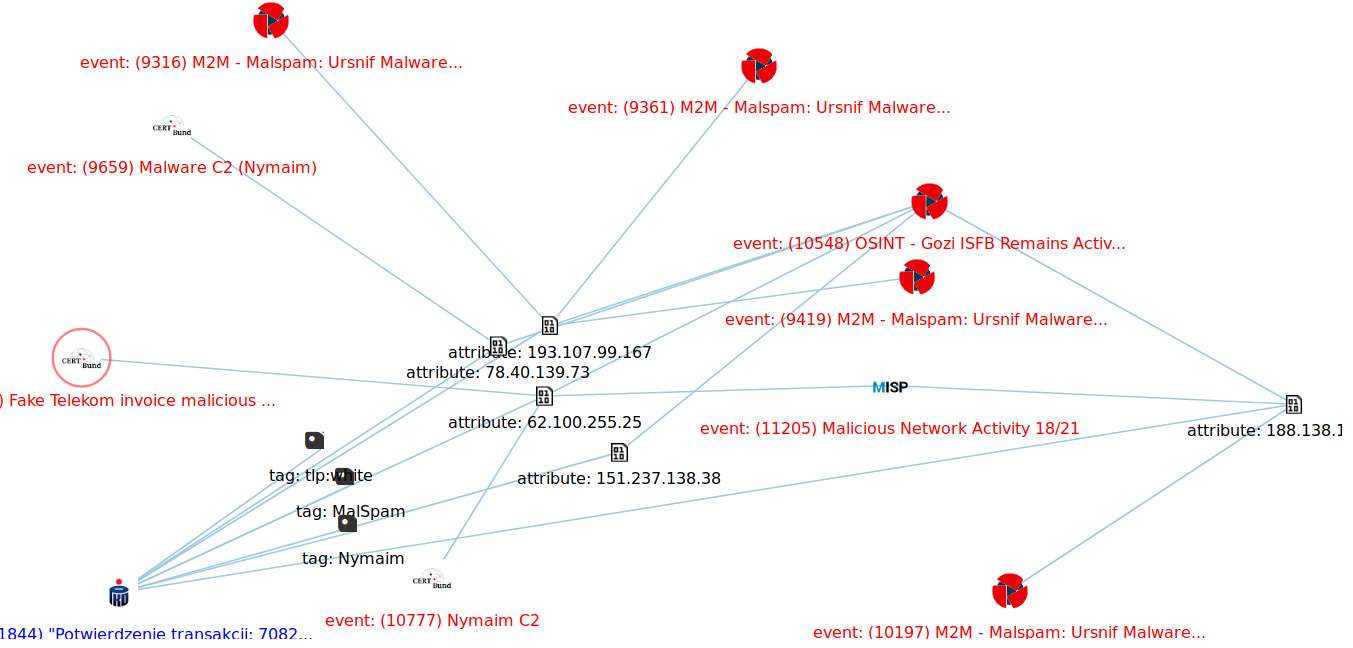
\includegraphics[scale=0.18]{screenshots/campaign.png}
        \end{center}
        \begin{itemize}
                \item To {\bf corroborate a finding} (e.g. is this the same campaign?), {\bf reinforce an analysis} (e.g. do other analysts have the same hypothesis?), {\bf confirm a specific aspect} (e.g. are the sinkhole IP addresses used for one campaign?) or just find if this {\bf threat is new or unknown in your community}.
        \end{itemize}
\end{frame}

\begin{frame}
        \frametitle{Contextualisation and aggregation}
        \begin{itemize}
                \item MISP integrates at the event and the attribute levels MITRE's Adversarial Tactics, Techniques, and Common Knowledge (ATT\&CK).
        \end{itemize}
        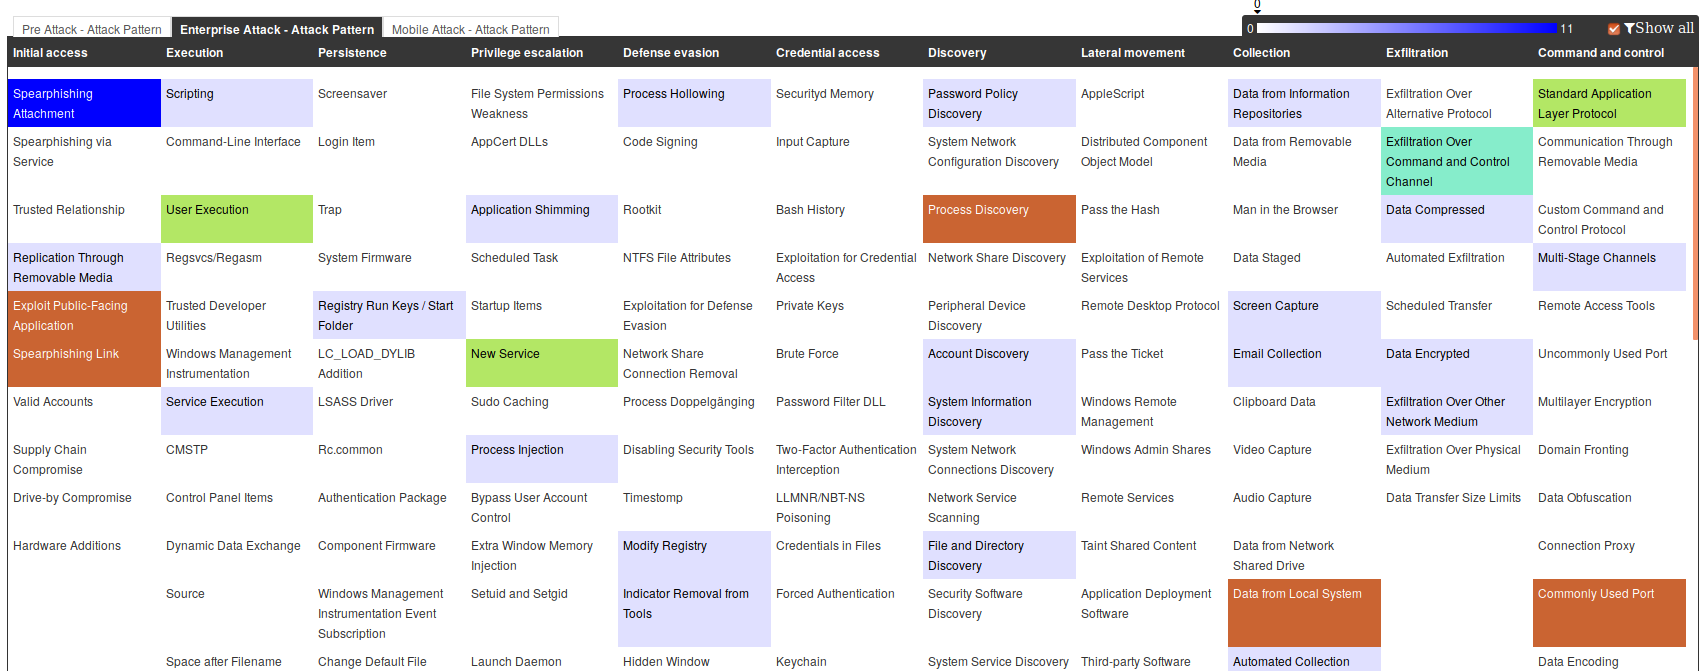
\includegraphics[scale=0.2]{screenshots/attack-screenshot.png}
\end{frame}

\begin{frame}
\frametitle{Sharing in MISP: Distribution}
    MISP offers granulars distribution settings
    \begin{itemize}
        \item Organisation only
        \item This community
        \item Connected communities
        \item All communities
        \item Distribution lists - aka {\bf Sharing groups}
    \end{itemize}
    \begin{center}
    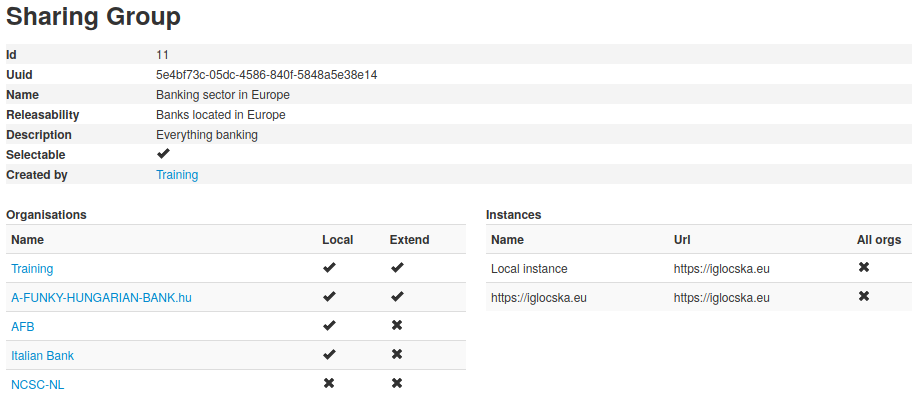
\includegraphics[scale=0.2]{screenshots/sg-example.png}
    \end{center}

    At multiple levels: Events, Attributes and Objects (and their Attributes)
\end{frame}

\begin{frame}
\frametitle{Sharing in MISP: Advanced usage}
    \begin{itemize}
        \item {\bf Delegation} for pseudo-anonymised information sharing
        \item {\bf Proposals} and {\bf Extended events} for collaborated information sharing
        \item 2-way synchronisation, Feed system, air-gapped sharing
        \item User defined {\bf filtered sharing} for all the above mentioned methods
        \item Cross-instance information {\bf caching} for quick lookups of large data-sets
        \item Support for multi-MISP internal enclaves
    \end{itemize}
\end{frame}

\begin{frame}
\frametitle{MISP core distributed sharing functionality}
    \begin{itemize}
        \item MISP's core functionality is sharing where everyone can be a consumer and/or a contributor/producer.
        \item Quick benefit without the obligation to contribute.
        \item Low barrier access to get acquainted to the system.
    \end{itemize}
    \begin{center}
        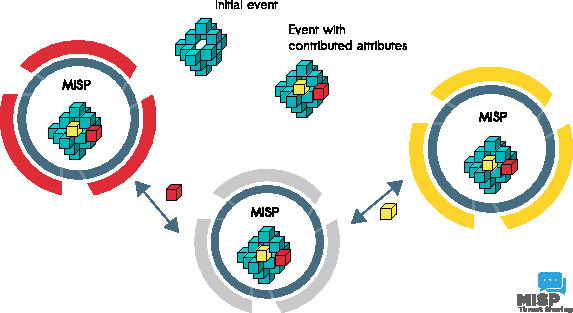
\includegraphics[scale=0.9]{misp-distributed.pdf}
    \end{center}
\end{frame}



\begin{frame}
\frametitle{Information quality management}
    \begin{itemize}
        \item Correlating data
        \item Feedback loop from detections via {\bf Sightings}
        \item {\bf False positive management} via the warninglist system
        \item {\bf Enrichment system} via MISP-modules
        \item {\bf Integrations} with a plethora of tools and formats
        \item Flexible {\bf API} and support {\bf libraries} such as PyMISP to ease integration
        \item {\bf Timelines} and giving information a temporal context
        \item Full chain for {\bf indicator life-cycle management}
    \end{itemize}
\end{frame}


\begin{frame}
        \frametitle{Sightings support}
        \begin{columns}[t]
        \column{5.0cm}
        \begin{figure}
        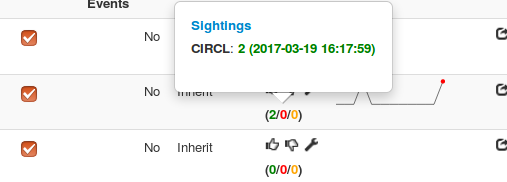
\includegraphics[scale=0.3]{screenshots/sighting-n.png}\\
        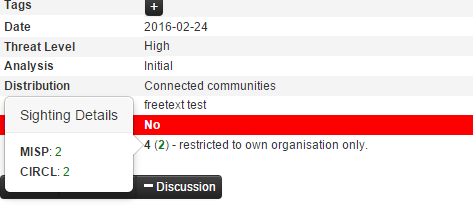
\includegraphics[scale=0.34]{screenshots/Sightings2.PNG}
        \end{figure}
        \column{7cm}
        \begin{itemize}
                \item \textit{Has a data-point been {\bf sighted} by me or the community before?}
                \item Additionally, the sighting system supports negative sigthings (FP) and expiration sightings.
                \item Sightings can be performed via the API or the UI.
                \item Many use-cases for {\bf scoring indicators} based on users sighting.
                \item For large quantities of data, {\bf SightingDB} by Devo
        \end{itemize}
        \end{columns}
\end{frame}

\begin{frame}
  \frametitle{Timelines and giving information a temporal context}
  \begin{itemize}
    \item Recently introduced {\bf \texttt{first\_seen}} and {\bf \texttt{last\_seen}} data points
    \item All data-points can be placed in time
    \item Enables the {\bf visualisation} and {\bf adjustment} of indicators timeframes 
  \end{itemize}
  \begin{center}
    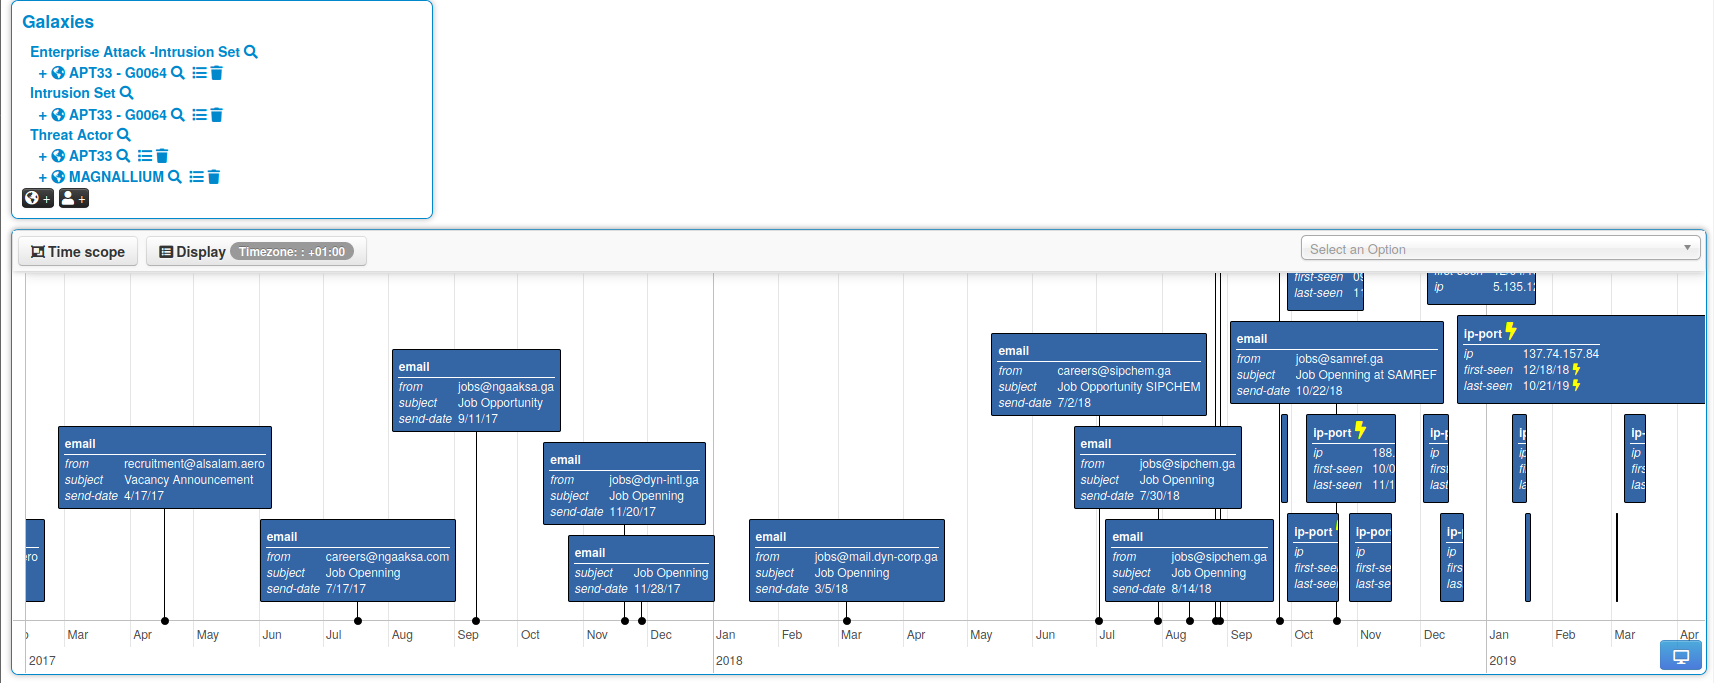
\includegraphics[width=1.0\linewidth]{timeline-misp-overview.png}
  \end{center}
\end{frame}

\begin{frame}
    \frametitle{Life-cycle management via decaying of indicators}
    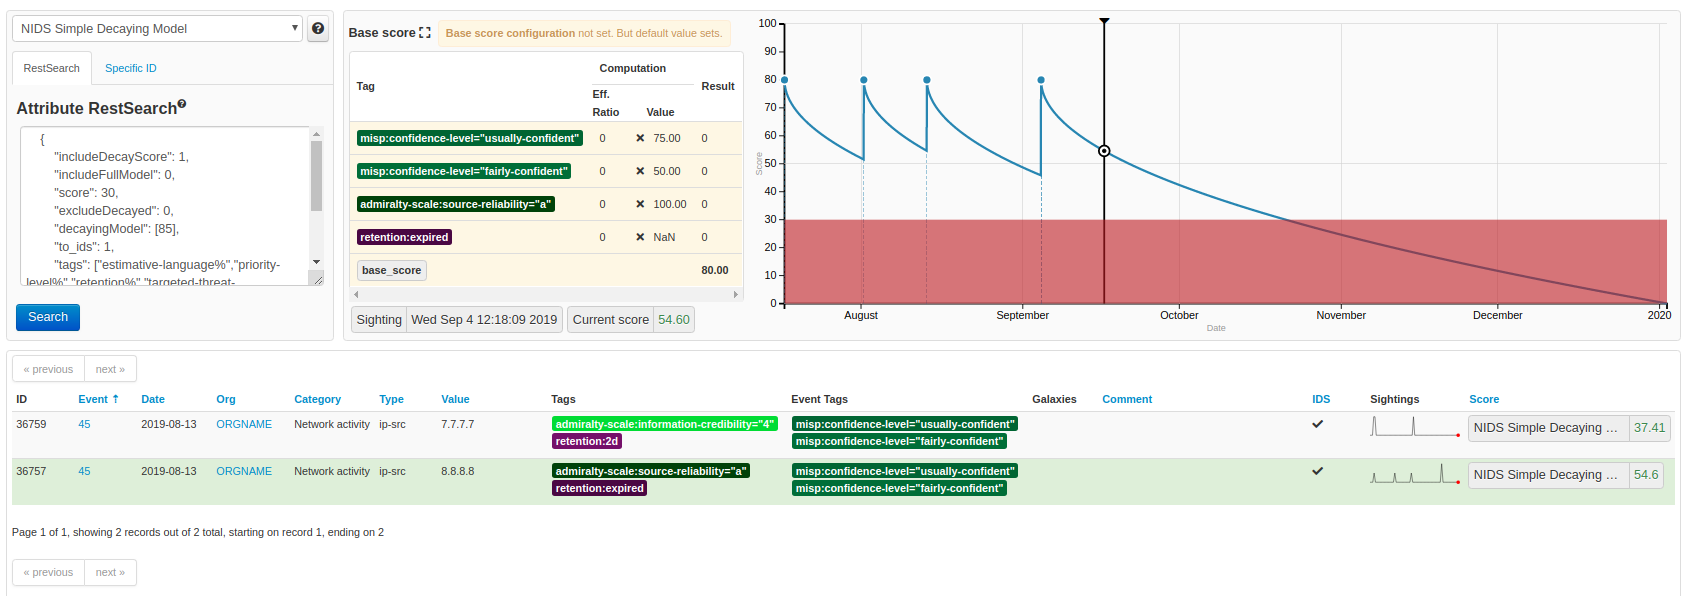
\includegraphics[width=1.00\linewidth]{decaying-simulation.png}
    Expiration based on user-defined \textit{Models}
\end{frame}

\begin{frame}
    \frametitle{GSMA specific {\bf taxonomies}}
    \begin{itemize}
        \item \texttt{gsma-attack-category}
        \begin{itemize}
            \item Used by GSMA for their information sharing program with telco describing the {\bf attack categories}
        \end{itemize}
        \item \texttt{gsma-fraud}
        \begin{itemize}
            \item Used by GSMA for their information sharing program with telco describing the {\bf various aspects of fraud}
        \end{itemize}
        \item \texttt{gsma-network-technology}
        \begin{itemize}
              \item Used by GSMA for their information sharing program with telco describing the {\bf types of infrastructure}.
        \end{itemize}
    \end{itemize}
\end{frame}


\begin{frame}
    \frametitle{Telco usefull {\bf galaxies}: Bhadra Framework}
    Bhadra is a threat modeling framework for mobile communication systems\footnote{https://arxiv.org/pdf/2005.05110.pdf}
    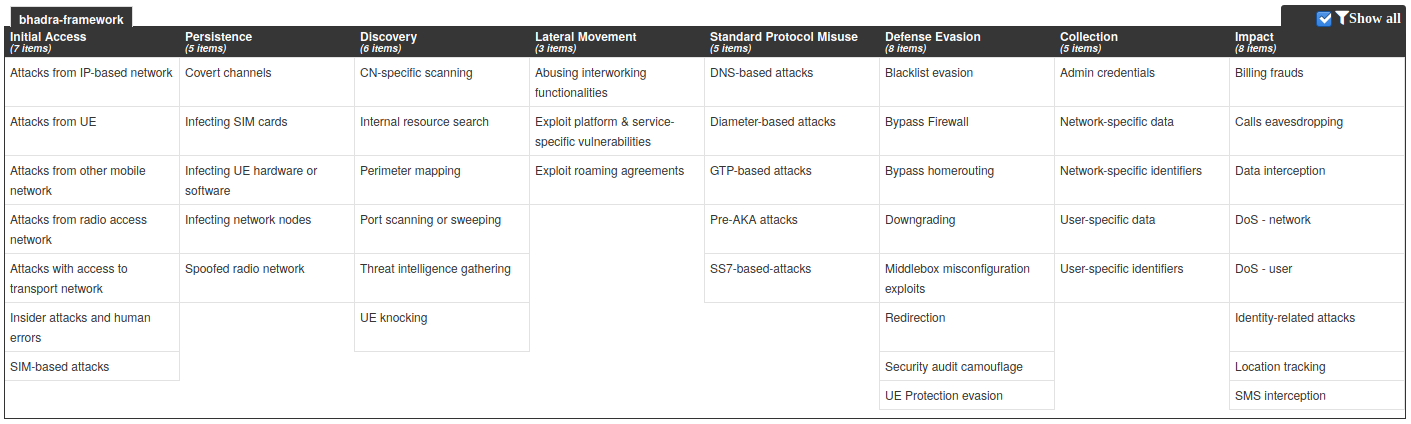
\includegraphics[width=1.05\linewidth]{screenshots/bhadra-matrix.png}
\end{frame}

\begin{frame}
    \frametitle{Telco usefull {\bf MISP Objects}}
    \begin{itemize}
        \item \texttt{phone}
        \begin{itemize}
            \item A phone or mobile phone object which describe a phone
            \item \texttt{brand}, \texttt{imei}, \texttt{imsi}, \texttt{serial-number}, ...
        \end{itemize}

        \item \texttt{short-message-service}
        \begin{itemize}
            \item Short Message Service (SMS) object template describing one or more SMS message
            \item \texttt{body}, \texttt{from}, \texttt{to}, \texttt{received-date}, ...
        \end{itemize}

        \item \texttt{ss7-attack}
        \begin{itemize}
            \item SS7 object of an attack seen on a GSM, UMTS or LTE network via SS7 logging
            \item \texttt{SccpCdGT}, \texttt{Category}, \texttt{MapOpCode}, ...
        \end{itemize}
    \end{itemize}
\end{frame}

\begin{frame}
    \frametitle{Acknowledgements}
    \begin{itemize}
        \item Supported by the grant \texttt{2018-LU-IA-0148}
        \item Pan-European Information Sharing \& Analysis fos IXP and GRX
        \item Goal is to create and support existing ISACs
        \begin{itemize}
            \item T-ISAC initiative of GSMA
            \item Internet Exchange Points (IXPs)
            \item General Packet Radio Service Roaming eXchange (GRXs)
            \item Network operators at large
        \end{itemize}
        \item Who is begind LU-CIX, Post Luxembourg and CIRCL
        \item \url{https://pisax.org/}
    \end{itemize}
    \begin{center}
        
\includegraphics[scale=0.5]{en_cef.png}
    \end{center}
\end{frame}


\begin{frame}
        \frametitle{Conclusion}
        \begin{itemize}
                \item {\bf Information sharing practices come from usage} and by example (e.g. learning by imitation from the shared information).
                \item MISP is just a tool. What matters is your sharing practices. The tool should be as transparent as possible to support you.
                \item Enable users to customize MISP to meet their community's use-cases.
                \item MISP project combines open source software, open standards, best practices and communities to make information sharing a reality.
        \end{itemize}
        \begin{center}
        
\includegraphics[scale=0.5]{en_cef.png}
        \end{center}
\end{frame}


